\documentclass[tikz,border=3pt,10pt]{standalone}

\usepackage{fontspec}
\usepackage{unicode-math}
\usepackage{pgfplots}
\pgfplotsset{compat=1.18}

\setmainfont{STIXTwoText-Regular.otf}[
  Path=../../../../../../../assets/fonts/,
  BoldFont=STIXTwoText-Bold.otf,
  ItalicFont=STIXTwoText-Italic.otf,
  BoldItalicFont=STIXTwoText-BoldItalic.otf
]
\setmathfont{STIXTwoMath.otf}[Path=../../../../../../../assets/fonts/]

\usetikzlibrary{backgrounds}

\definecolor{zoPlotBackground}{HTML}{FFF9E9}
\definecolor{zoPlotBorder}{HTML}{DFD7CA}
\definecolor{zoAxis}{HTML}{554F48}
\definecolor{zoText}{HTML}{3E3A35}
\definecolor{zoGraphMain}{HTML}{EF5350}
\definecolor{zoHighlightLight}{HTML}{FFF4D4}

\pgfplotsset{
  zo axis/.style={
    width=12cm,
    height=7.5cm,
    scale only axis,
    axis equal image=false,
    enlargelimits=false,
    clip=true,
    clip mode=individual,
    axis lines=middle,
    grid=none,
    axis line style={draw=zoAxis,line width=0.8pt,<->},
    tick align=center,
    tickwidth=0.4mm,
    tick style={draw=zoAxis,line width=0.32pt},
    every axis plot/.append style={line cap=round,line join=round}
  },
  zo graph main/.style={
    draw=zoGraphMain,
    line width=1.2pt,
    solid,
    no marks
  }
}

\tikzset{
  zo graph field/.style={
    show background rectangle,
    inner frame sep=4mm,
    background rectangle/.style={
      fill=zoPlotBackground,
      draw=zoPlotBorder,
      line width=0.45pt,
      rounded corners=2mm
    }
  },
  zo graph label/.style={
    text=zoText,
    font=\small
  }
}

\begin{document}
\begin{tikzpicture}[zo graph field]
  \begin{axis}[
    zo axis,
    width=14cm,
    height=7cm,
    axis x line=bottom,
    axis y line=left,
    axis line style={draw=zoAxis,line width=0.8pt,->},
    xmin=0,
    xmax=8.5,
    ymin=0,
    ymax=1.25,
    xtick={1,2,4,8},
    ytick={1},
    xticklabel=\empty,
    yticklabel=\empty
  ]
    % Ba miền có cùng tỉ lệ đầu mút và cùng diện tích ln 2.
    \addplot[
      draw=none,
      fill=zoHighlightLight,
      fill opacity=0.92,
      domain=1:2,
      samples=80
    ] {1/x} \closedcycle;
    \addplot[
      draw=none,
      fill=zoHighlightLight,
      fill opacity=0.92,
      domain=2:4,
      samples=80
    ] {1/x} \closedcycle;
    \addplot[
      draw=none,
      fill=zoHighlightLight,
      fill opacity=0.92,
      domain=4:8,
      samples=100
    ] {1/x} \closedcycle;

    \draw[draw=zoAxis,line width=0.6pt,densely dashed]
      (axis cs:1,0) -- (axis cs:1,1);
    \draw[draw=zoAxis,line width=0.6pt,densely dashed]
      (axis cs:2,0) -- (axis cs:2,0.5);
    \draw[draw=zoAxis,line width=0.6pt,densely dashed]
      (axis cs:4,0) -- (axis cs:4,0.25);
    \draw[draw=zoAxis,line width=0.6pt,densely dashed]
      (axis cs:8,0) -- (axis cs:8,0.125);

    % Mở rộng miền lấy mẫu để đường cong đi vào từ biên trên và ra khỏi biên phải.
    \addplot[
      zo graph main,
      domain=0.75:8.6,
      samples=500
    ] {1/x};

    \node[
      text=zoText,
      font=\footnotesize,
      anchor=north,
      yshift=-2pt
    ] at (axis cs:1,0) {$1$};
    \node[
      text=zoText,
      font=\footnotesize,
      anchor=north,
      yshift=-2pt
    ] at (axis cs:2,0) {$2$};
    \node[
      text=zoText,
      font=\footnotesize,
      anchor=north,
      yshift=-2pt
    ] at (axis cs:4,0) {$4$};
    \node[
      text=zoText,
      font=\footnotesize,
      anchor=north,
      yshift=-2pt
    ] at (axis cs:8,0) {$8$};
    \node[
      text=zoText,
      font=\footnotesize,
      anchor=east,
      xshift=-2pt
    ] at (axis cs:0,1) {$1$};

    \node[zo graph label] at (axis cs:1.43,0.23) {$\ln 2$};
    \node[zo graph label] at (axis cs:2.85,0.15) {$\ln 2$};
    \node[zo graph label] at (axis cs:5.7,0.09) {$\ln 2$};
    \node[
      zo graph label,
      anchor=south west,
      xshift=2pt,
      yshift=2pt
    ] at (axis cs:5.2,{1/5.2}) {$y=\dfrac{1}{t}$};

    \node[
      text=zoText,
      font=\normalsize,
      anchor=west,
      xshift=3pt
    ] at (axis cs:8.5,0) {$t$};
    \node[
      text=zoText,
      font=\normalsize,
      anchor=south,
      yshift=3pt
    ] at (axis cs:0,1.25) {$y$};
  \end{axis}
\end{tikzpicture}
\end{document}
